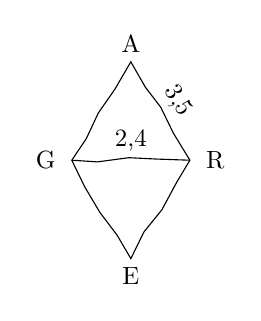
\begin{tikzpicture}[rotate=0,every node/.style={scale=0.9},scale=1]

\coordinate (G) at (0,0);
\coordinate (A) at (0.75,1.25);
\coordinate (R) at (1.5,0);
\coordinate (E) at (0.75,-1.25);

\draw[decorate,decoration={random steps,amplitude=1pt,segment length=10pt}] (G) node [left=3pt]{G}--(A) node [above]{A}--(R) node [right=3pt] {R}--(E) node [below] {E}--cycle;
\draw [decorate,decoration={random steps,amplitude=1pt,segment length=10pt}] (G)--(R);
\path (A)--(R) node[midway,above,sloped]{3,5};
\path (G)--(R) node[midway,above]{2,4};

\end{tikzpicture}